% Present results
% Explain results

In this section, we discuss the computational efficiency of our implementation of WHVI and FWHT\@.
The regression experiments were run on Linux Ubuntu 20.04 with an Intel I7-6700K CPU and a GeForce GTX 970 GPU\@.

It is not clear from the original paper to what extent the in-place version of FWHT was utilized.
We found that using in-place operations caused problems in the PyTorch automatic differentiation engine so that the computed gradient was incorrect.
We consequently cloned the input batch before using the transform, but this did not noticeably decrease processing speed.

The CUDA implementation of FWHT was not explained in the original paper or the supplement.
We adapted an implementation of the kernel from the original paper\footnote{See the paper's repository at \url{https://github.com/srossi93/vardl} and a different implementation of the transform at \url{https://github.com/HazyResearch/structured-nets}.} and used it in our experiments.
We suggest the paper by Bikov and Bouyukliev (2018)~\cite{bikov2018parallel} for a clear and concise FWHT implementation reference, as well as the detailed implementation strategies, described by Arndt (2010)~\cite{arndt2010matters}.

The following benchmarks were run on Windows 10 with an AMD Ryzen 9 3900X CPU and a GeForce RTX 2070S GPU\@.
We noticed that using a non-vectorized Python/C++ CPU implementation of FWHT yielded consistently slower results than matrix multiplication on the CPU with no sign of change.
However, a vectorized Python implementation yields the same results as those in the original paper, i.e.\ the tradeoff point occurs at approximately $D = 2^{11}$.
The results are shown in Figure~\ref{fig:compute-performance}.

\begin{figure}[htb]
    \centering
    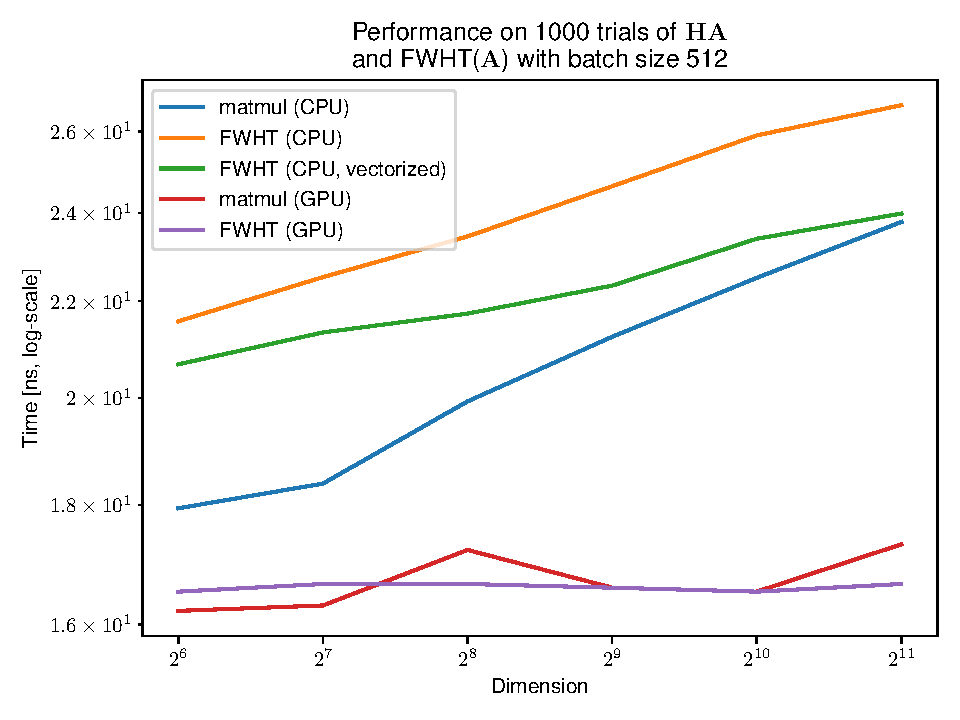
\includegraphics[width=\hsize]{img/compute-performance-all}
    \caption{
        FWHT and matrix multiplication performance comparison on the CPU and GPU.
        Results are based on 1000 transformations of 512 vectors with standard normal random entries, each vector consisting of $D$ elements (shown as ``Dimension'' on the $x$-axis).
        The vectors are arranged into the matrix $\mathbf{A}$.
        The vectorized CPU implementation beats matrix multiplication at around $D = 2^{11}$ in compute time, but the non-vectorized implementation is consistently worse.
        Both operations are much faster on the GPU, and FWHT outperforms matrix multiplications at moderate values of $D$.
        These results agree with the ones in the Supplement for the original paper.
    }
    \label{fig:compute-performance}
\end{figure}
